\section{Diskussion}
De tre simulerede programkørsler rand, scan og focus er blevet kørt 100 gange med de tre forskellige sideudskiftningsalgoritmer. Der er samlet statistik over hvor mange disktilgange, de forskellige algoritmer har med et skiftende antal fysiske sider. Programkørslerne resulterede i meget forskellig opførsel i antallet af disk tilgange. I dette afsnit beskrives diskuteres de forskellige resultater, alle kørslerne i en graf kan ses i figur \ref{fig:all}.

\begin{figure}[ht]
\centerline{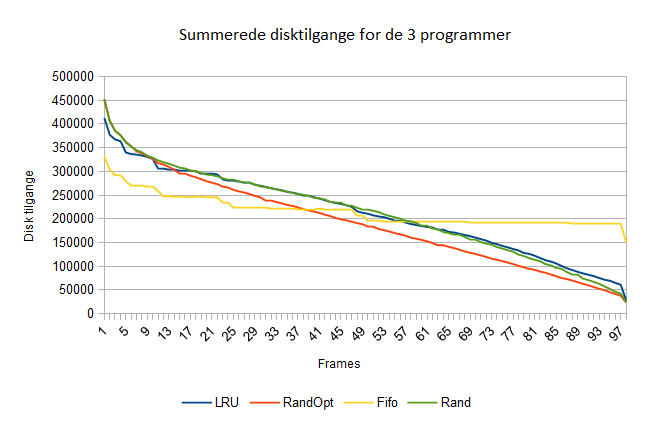
\includegraphics[scale=1]{graph/stat_all}}
\FloatBarrier
\caption{Alle kørsler summeret}
\label{fig:all}
\end{figure}

\subsubsection{Sekventielle løb}
Programmet "Scan" består af 10 sekventielle løb gennem alt data. Det kan  hverken FIFO eller LRU håndtere særlig godt, da begge algoritmer bygger på den antagelse at der er størst sandsynlighed for at data der lige er blevet brugt, snart skal bruges igen. Ved sekventielle gennemløb er det det omvendte der er tilfældet. 

\begin{figure}[ht]
\centerline{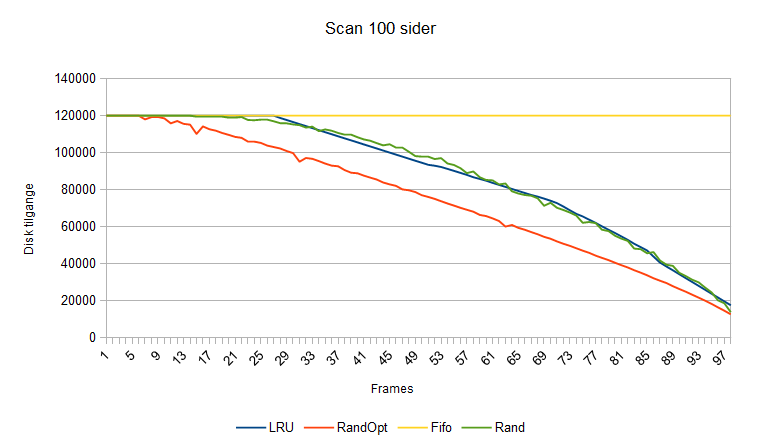
\includegraphics[scale=1]{graph/stat_scan}}
\FloatBarrier
\caption{Alle kørsler summeret}
\label{fig:scan}
\end{figure}

\subsubsection{Rand}

\subsubsection{Custom}

\subsubsection{RandOpt}

\subsection{Diskussion af resultater}
At rand algoritmen er den hurtigste er en gåde for os....!
